\ifx\allfiles\undefined
\documentclass[12pt, a4paper, oneside, UTF8]{ctexbook}
\def\path{../config}
\usepackage{amsmath}
\usepackage{amsthm}
\usepackage{array}
\usepackage{amssymb}
\usepackage{graphicx}
\usepackage{mathrsfs}
\usepackage{enumitem}
\usepackage{geometry}
\usepackage[colorlinks, linkcolor=black]{hyperref}
\usepackage{stackengine}
\usepackage{yhmath}
\usepackage{extarrows}
% \usepackage{unicode-math}
\usepackage{esint}
\usepackage{multirow}
\usepackage{fancyhdr}
\usepackage[dvipsnames, svgnames]{xcolor}
\usepackage{listings}
\usepackage{float} % Required for the H float option
\definecolor{mygreen}{rgb}{0,0.6,0}
\definecolor{mygray}{rgb}{0.5,0.5,0.5}
\definecolor{mymauve}{rgb}{0.58,0,0.82}
\definecolor{NavyBlue}{RGB}{0,0,128}
\definecolor{Rhodamine}{RGB}{255,0,255}
\definecolor{PineGreen}{RGB}{0,128,0}

\graphicspath{ {figures/},{../figures/}, {config/}, {../config/} }

\linespread{1.6}

\geometry{
    top=25.4mm, 
    bottom=25.4mm, 
    left=20mm, 
    right=20mm, 
    headheight=2.17cm, 
    headsep=4mm, 
    footskip=12mm
}

\setenumerate[1]{itemsep=5pt,partopsep=0pt,parsep=\parskip,topsep=5pt}
\setitemize[1]{itemsep=5pt,partopsep=0pt,parsep=\parskip,topsep=5pt}
\setdescription{itemsep=5pt,partopsep=0pt,parsep=\parskip,topsep=5pt}

\lstset{
    language=Mathematica,
    basicstyle=\tt,
    breaklines=true,
    keywordstyle=\bfseries\color{NavyBlue}, 
    emphstyle=\bfseries\color{Rhodamine},
    commentstyle=\itshape\color{black!50!white}, 
    stringstyle=\bfseries\color{PineGreen!90!black},
    columns=flexible,
    numbers=left,
    numberstyle=\footnotesize,
    frame=tb,
    breakatwhitespace=false,
} 

\lstset{
    language=TeX, % 设置语言为 TeX
    basicstyle=\ttfamily, % 使用等宽字体
    breaklines=true, % 自动换行
    keywordstyle=\bfseries\color{NavyBlue}, % 关键字样式
    emphstyle=\bfseries\color{Rhodamine}, % 强调样式
    commentstyle=\itshape\color{black!50!white}, % 注释样式
    stringstyle=\bfseries\color{PineGreen!90!black}, % 字符串样式
    columns=flexible, % 列的灵活性
    numbers=left, % 行号在左侧
    numberstyle=\footnotesize, % 行号字体大小
    frame=tb, % 顶部和底部边框
    breakatwhitespace=false % 不在空白处断行
}

% \begin{lstlisting}[language=TeX] ... \end{lstlisting}

% 定理环境设置
\usepackage[strict]{changepage} 
\usepackage{framed}

\definecolor{greenshade}{rgb}{0.90,1,0.92}
\definecolor{redshade}{rgb}{1.00,0.88,0.88}
\definecolor{brownshade}{rgb}{0.99,0.95,0.9}
\definecolor{lilacshade}{rgb}{0.95,0.93,0.98}
\definecolor{orangeshade}{rgb}{1.00,0.88,0.82}
\definecolor{lightblueshade}{rgb}{0.8,0.92,1}
\definecolor{purple}{rgb}{0.81,0.85,1}

\theoremstyle{definition}
\newtheorem{myDefn}{\indent Definition}[section]
\newtheorem{myLemma}{\indent Lemma}[section]
\newtheorem{myThm}[myLemma]{\indent Theorem}
\newtheorem{myCorollary}[myLemma]{\indent Corollary}
\newtheorem{myCriterion}[myLemma]{\indent Criterion}
\newtheorem*{myRemark}{\indent Remark}
\newtheorem{myProposition}{\indent Proposition}[section]

\newenvironment{formal}[2][]{%
	\def\FrameCommand{%
		\hspace{1pt}%
		{\color{#1}\vrule width 2pt}%
		{\color{#2}\vrule width 4pt}%
		\colorbox{#2}%
	}%
	\MakeFramed{\advance\hsize-\width\FrameRestore}%
	\noindent\hspace{-4.55pt}%
	\begin{adjustwidth}{}{7pt}\vspace{2pt}\vspace{2pt}}{%
		\vspace{2pt}\end{adjustwidth}\endMakeFramed%
}

\newenvironment{definition}{\vspace{-\baselineskip * 2 / 3}%
	\begin{formal}[Green]{greenshade}\vspace{-\baselineskip * 4 / 5}\begin{myDefn}}
	{\end{myDefn}\end{formal}\vspace{-\baselineskip * 2 / 3}}

\newenvironment{theorem}{\vspace{-\baselineskip * 2 / 3}%
	\begin{formal}[LightSkyBlue]{lightblueshade}\vspace{-\baselineskip * 4 / 5}\begin{myThm}}%
	{\end{myThm}\end{formal}\vspace{-\baselineskip * 2 / 3}}

\newenvironment{lemma}{\vspace{-\baselineskip * 2 / 3}%
	\begin{formal}[Plum]{lilacshade}\vspace{-\baselineskip * 4 / 5}\begin{myLemma}}%
	{\end{myLemma}\end{formal}\vspace{-\baselineskip * 2 / 3}}

\newenvironment{corollary}{\vspace{-\baselineskip * 2 / 3}%
	\begin{formal}[BurlyWood]{brownshade}\vspace{-\baselineskip * 4 / 5}\begin{myCorollary}}%
	{\end{myCorollary}\end{formal}\vspace{-\baselineskip * 2 / 3}}

\newenvironment{criterion}{\vspace{-\baselineskip * 2 / 3}%
	\begin{formal}[DarkOrange]{orangeshade}\vspace{-\baselineskip * 4 / 5}\begin{myCriterion}}%
	{\end{myCriterion}\end{formal}\vspace{-\baselineskip * 2 / 3}}
	

\newenvironment{remark}{\vspace{-\baselineskip * 2 / 3}%
	\begin{formal}[LightCoral]{redshade}\vspace{-\baselineskip * 4 / 5}\begin{myRemark}}%
	{\end{myRemark}\end{formal}\vspace{-\baselineskip * 2 / 3}}

\newenvironment{proposition}{\vspace{-\baselineskip * 2 / 3}%
	\begin{formal}[RoyalPurple]{purple}\vspace{-\baselineskip * 4 / 5}\begin{myProposition}}%
	{\end{myProposition}\end{formal}\vspace{-\baselineskip * 2 / 3}}


\newtheorem{example}{\indent \color{SeaGreen}{Example}}[section]
\renewcommand{\proofname}{\indent\textbf{\textcolor{TealBlue}{Proof}}}
\newenvironment{solution}{\begin{proof}[\indent\textbf{\textcolor{TealBlue}{Solution}}]}{\end{proof}}

% 自定义命令的文件

\def\d{\mathrm{d}}
\def\R{\mathbb{R}}
%\newcommand{\bs}[1]{\boldsymbol{#1}}
%\newcommand{\ora}[1]{\overrightarrow{#1}}
\newcommand{\myspace}[1]{\par\vspace{#1\baselineskip}}
\newcommand{\xrowht}[2][0]{\addstackgap[.5\dimexpr#2\relax]{\vphantom{#1}}}
\newenvironment{mycases}[1][1]{\linespread{#1} \selectfont \begin{cases}}{\end{cases}}
\newenvironment{myvmatrix}[1][1]{\linespread{#1} \selectfont \begin{vmatrix}}{\end{vmatrix}}
\newcommand{\tabincell}[2]{\begin{tabular}{@{}#1@{}}#2\end{tabular}}
\newcommand{\pll}{\kern 0.56em/\kern -0.8em /\kern 0.56em}
\newcommand{\dive}[1][F]{\mathrm{div}\;\boldsymbol{#1}}
\newcommand{\rotn}[1][A]{\mathrm{rot}\;\boldsymbol{#1}}

% 修改参数改变封面样式,0 默认原始封面、内置其他1、2、3种封面样式
\def\myIndex{0}


\ifnum\myIndex>0
    \input{\path/cover_package_\myIndex}
\fi

\def\myTitle{标题:一份LaTeX笔记模板}
\def\myAuthor{作者名称}
\def\myDateCover{封面日期: \today}
\def\myDateForeword{前言页显示日期: \today}
\def\myForeword{前言标题}
\def\myForewordText{
    
    这是一个基于\LaTeX{}的模板,用于撰写学习笔记。

    模板旨在提供一个简单、易用的框架,以便你能够专注于内容,而不是排版细节,如不是专业者,不建议使用者在模板细节上花费太多时间,而是直接使用模板进行笔记撰写。遇到问题,再进行调整解决。
}
\def\mySubheading{副标题}


\begin{document}
% \input{\path/cover_text_\myIndex.tex}

\newpage
\thispagestyle{empty}
\begin{center}
    \Huge\textbf{\myForeword}
\end{center}
\myForewordText
\begin{flushright}
    \begin{tabular}{c}
        \myDateForeword
    \end{tabular}
\end{flushright}

\newpage
\pagestyle{plain}
\setcounter{page}{1}
\pagenumbering{Roman}
\tableofcontents

\newpage
\pagenumbering{arabic}
\setcounter{chapter}{-1}
\setcounter{page}{1}

\pagestyle{fancy}
\fancyfoot[C]{\thepage}
\renewcommand{\headrulewidth}{0.4pt}
\renewcommand{\footrulewidth}{0pt}








\else
\fi

\chapter{侧压力}

\section{土压力}
\begin{definition}
    根据挡土墙的位移情况和墙后土体所处的平衡状态,将土压力分为:静止土压力、主动土压力和被动土压力
\end{definition}

\begin{figure}[H]
    \centering
    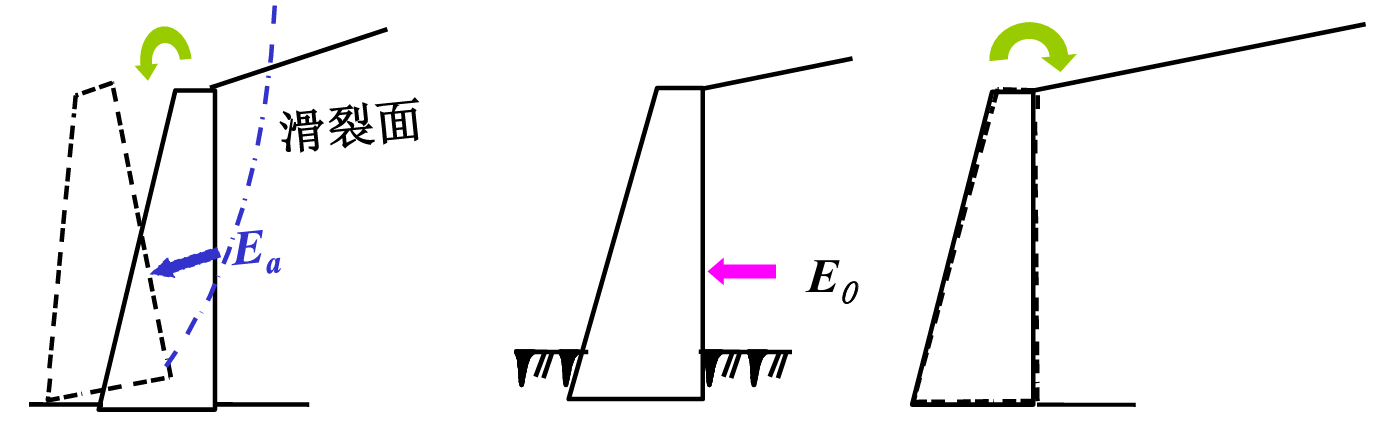
\includegraphics[width=0.8\textwidth]{../figure/dangtuqiang.png}
    \caption{土压力分类}
\end{figure}

\begin{enumerate}
    \item 挡土墙{\color{red}没有任何变形和位移},墙后土体处于{\color{red}弹性平衡状态},该
    状态下作用在挡土墙上的土压力就称为静止土压力,比如地下室,记为$E_0$
    \item 挡土墙{\color{red}向背离土体的方向发生位移},此时土压力会不断减小,
当土体达到极限状态时,该状态下作用在挡土墙上的土压力就
称为主动土压力,比如说基坑,记为$E_a$
    \item 挡土墙朝{\color{red}向土体方向发生位移},此时土压力会不断增大,当土
    体达到极限状态时,该状态下作用在挡土墙上的土压力就称为被动土压力,比如说拱桥,记为$E_p$
\end{enumerate}

{\color{red}这里部分的推导有点简略了,我在考试前又写了一遍,可以看笔记最后一章计算题与易错题部分。}

\begin{remark}
    $
    E_p>E_0>E_a
    $
\end{remark}

\begin{definition}
    由朗肯土压力理论,土体中某点处于极限平衡状态,可导出大、小主应力之间的关系式:

粘性土
$$
\sigma_1 = \sigma_3 \tan^2 \left( 45^\circ + \frac{\phi}{2} \right) + 2c \tan \left( 45^\circ + \frac{\phi}{2} \right)
$$
$$
\sigma_3 = \sigma_1 \tan^2 \left( 45^\circ - \frac{\phi}{2} \right) - 2c \tan \left( 45^\circ - \frac{\phi}{2} \right)
$$

无粘性土
$$
\sigma_1 = \sigma_3 \tan^2 \left( 45^\circ + \frac{\phi}{2} \right)
$$
$$
\sigma_3 = \sigma_1 \tan^2 \left( 45^\circ - \frac{\phi}{2} \right)
$$
\end{definition}

\begin{figure}[H]
    \centering
    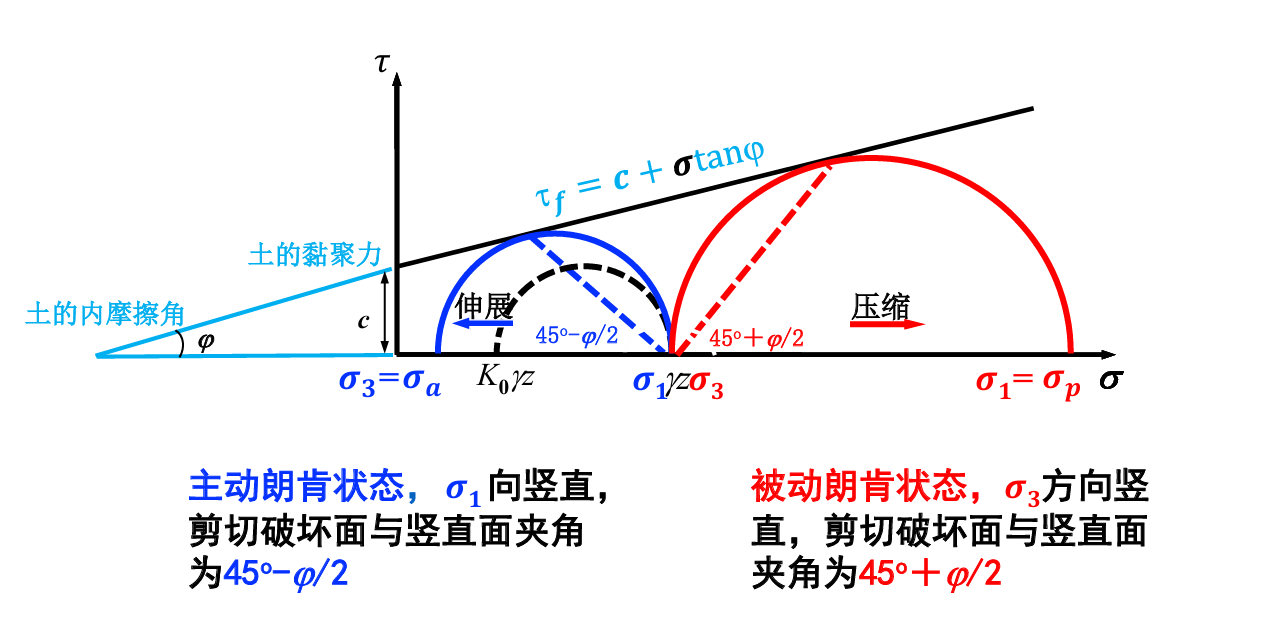
\includegraphics[width=0.8\textwidth]{../figure/tuceyali.png}
    \caption{莫尔圆}
\end{figure}

\begin{definition}
    由朗肯土压力理论,土体中某点处于极限平衡状态,可导出大、小主应力之间的关系式:

记$K_p = \tan^2 \left( 45^\circ + \frac{\phi}{2} \right)$,$K_a = \tan^2 \left( 45^\circ - \frac{\phi}{2} \right)$,而$\gamma z$就是静止土压力

粘性土
$$
\sigma_p = \gamma z K_p + 2c \sqrt{K_p}
$$
被动土压力
$$
\sigma_a = \gamma z K_a - 2c \sqrt{K_a}
$$
主动土压力

无粘性土
$$
\sigma_p = \gamma z K_p
$$
被动土压力
$$
\sigma_a = \gamma z K_a
$$
主动土压力
\end{definition}

\begin{remark}
    粘性土产生的等效高度为$\frac{2c}{\gamma \sqrt{K}}$

    如果是主动土压力的话,粘性土起到拉拽的效果。
    如果是被动土压力的话,粘性土起到压缩的效果。
\end{remark}

\begin{figure}[H]
    \centering
    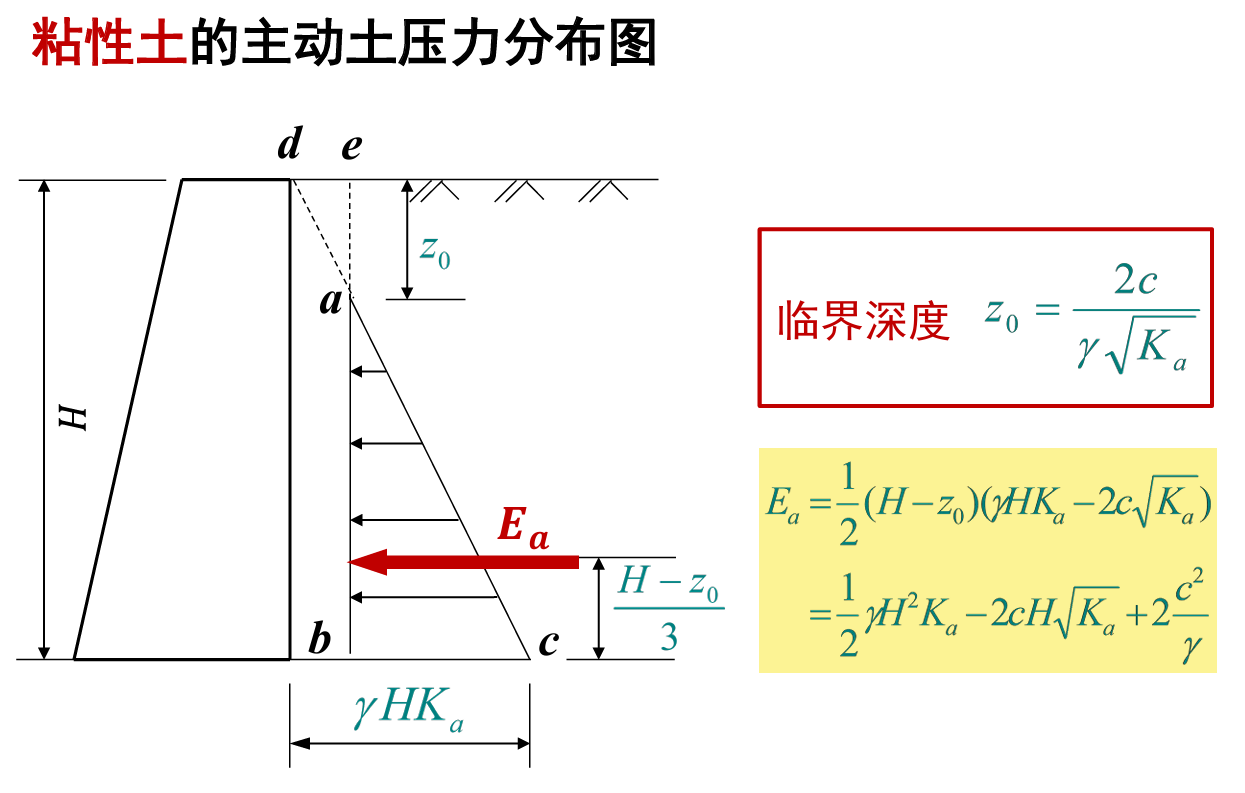
\includegraphics[width=0.8\textwidth]{../figure/zhudong.png}
    \caption{主动土压力}
\end{figure}

\begin{figure}[H]
    \centering
    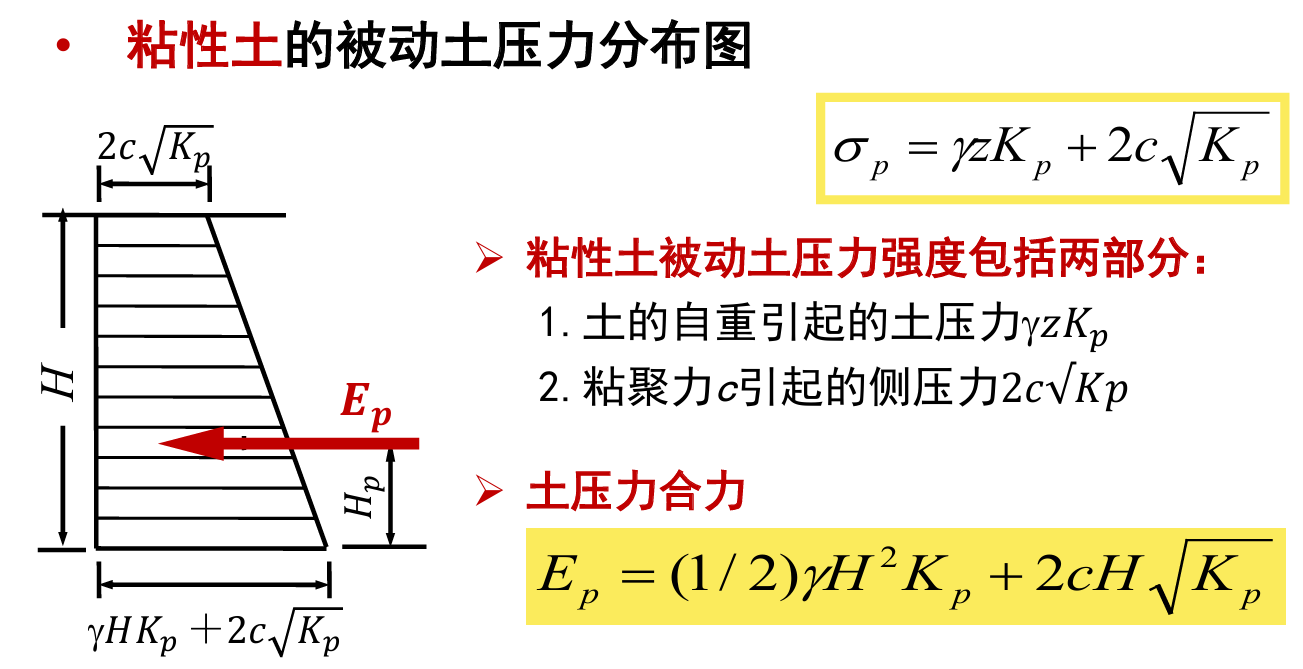
\includegraphics[width=0.8\textwidth]{../figure/beidong.png}
    \caption{被动土压力}
\end{figure}

\section{水压力}

水对结构的作用包括化学作用与物理作用;

1. 化学作用表现为水对结构的腐蚀或侵蚀作用;

2. 物理作用表现为水对结构的力学作用,即水对结构表面产生的静压力和动压力。

\begin{definition}
\[
p = p_{\text{静}} + p_{\text{动}}
\]
\[
p = p_{\text{静}} + \bar{p_{\text{动}}} + p_{\text{动}}^{\prime}
\]  
解释下,这里是采用了流体力学的处理方法,将流水压力分解为动水压力和静水压力两部分。其中
动水压力又分解为时段平均动压力和脉动压力。
\end{definition}

\begin{remark}
    实际计算中\( p'_{\text{动}} \)采用较大的可能值,一般取3-5倍的脉动标准差动。水压力还可能引起结构振动,在结构设计时,必须加以考虑。
\end{remark}

\begin{example}
    在水流过结构物表面时,会对结构物产生切应力和正应力,切应力与水流的方向一致,且只有在水低速流动时才表现出来。(错,实际上切应力与水流的方向平行,且只有在水高速流动时才表现出来。)
\end{example}

\section{波浪荷载}

\begin{figure}[H]
    \centering
    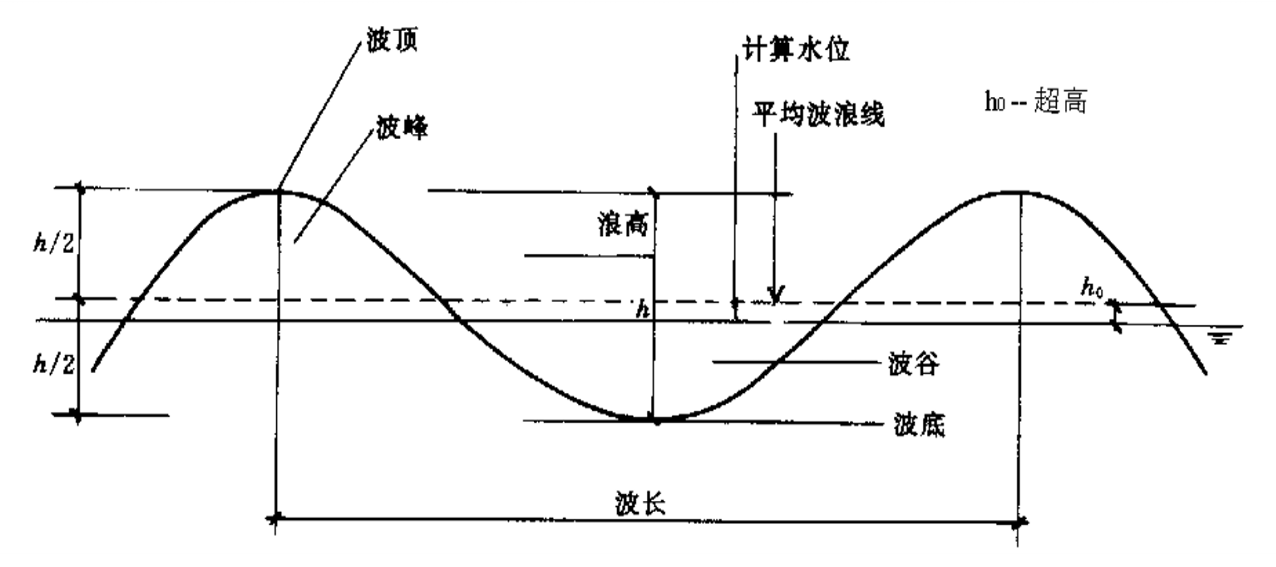
\includegraphics[width=0.6\textwidth]{../figure/bol.png}
    \caption{波浪荷载示意图}
\end{figure}

\begin{definition}
    波浪在干扰力的作用下生成:
    \begin{itemize}
        \item 由风力引起的波浪称为\textbf{风成波}
        \item 由月球引力引起的波浪称为\textbf{潮汐波}
        \item 由船舶航行引起的波浪称为\textbf{船行波}
        \item 由海底地震引起的波浪称为\textbf{海啸}
    \end{itemize}
\end{definition}

对港口建筑和水工结构来说,风成波影响最大,是工程设计主要考虑对象。

\begin{definition}
    波高和波长的比值$h/\lambda$称波陡

    平分波高的水平线称波浪中线

    波浪中线到静止水面的垂直距离称超高,用$h_0$表示

    波顶向前推进一个波长所需的时间称波周期,用$T$表示。
\end{definition}

\subsection{波浪的传播过程}

在海洋深水区($d > \frac{L}{2}$),波浪运动不受海底摩擦阻力影响,称为\textbf{深水推进波}。

在海洋浅水区($d < \frac{L}{2}$),海底对波浪运动产生摩阻作用,称为\textbf{浅水推进波}。

当浅水波继续向海岸推进时,波陡相应增大,波峰发生破碎,这个区域称为\textbf{波浪破碎带}。

浅水推进波破碎后,又重新组成新的波浪向前推进,几度破碎,形成一股水流向前推移,这种波浪称为\textbf{击岸波}。

击岸波形成的冲击水流即为\textbf{波浪荷载}。

现行确定波浪荷载的方法带有很大的经验性,一般情况下当浪高超过0.5m时,应考虑波浪对构筑物的作用力。

\begin{corollary}
    直墙上波浪荷载应按三种波浪进行设计:

(1)立波——原始推进波冲击垂直墙面后和反射波互相叠加形成的一种干涉波,只有上下运动而没有水平方向运动;

(2)近堤破碎波——距直墙附近半个波长范围内发生破碎的波;

(3)远堤破碎波——距直墙半个波长以外发生破碎的波。
\end{corollary}

\section{冻胀力}

\begin{definition}
    冻土:

    具有负温度或零温度,其中含有冰、水汽、液态水,且胶结着松散固体颗粒的土。

    冻土是多相天然复合体,是非均质、各向异性的多孔介质
\end{definition}

\begin{corollary}
    土的冻胀原理和效应
    \begin{enumerate}
        \item 冻土抵抗外力的强度提高
        \item 地基土冻结时产生冻胀,融化时产生融陷。这样的变形在受到结构物约束时,引起结构发生变形和产生内力。
        \item 主要表现在冬季低温时结构物开裂、断裂,严重者造成结构物倾覆等;春融期间地基沉降,对结构产生变形作用的附加荷载。
    \end{enumerate}
\end{corollary}

\begin{enumerate}
    \item {\color{red}颗粒越细冻胀越强},如粉性土冻胀最强烈
    \item 土体冻结时,土颗粒之间相互隔离,产生位移,使土体体
    积产生不均匀膨胀。
    \item 当冻胀力达到一定界限时,就不再产生冻胀,这时的冻胀力就
    是{\color{red}最大冻胀力}。
    \item 土体的冻胀及其特性既受到土颗粒大小的影响,也受
    到土颗粒外形的影响。
    \item {\color{red}含水量越大,地下水位越高,冻胀程度越大}。
\end{enumerate}

\begin{remark}
    作业题:叙述土的冻胀原理(简洁版本,下面是完整版本)

    冻胀原理:水体向冻结锋面迁移,使在冻结面上形成了冰夹层和冰透镜体,导致冻层膨胀,地层隆起。同时土体冻结时,土颗粒之间相互隔离,产生位移,使土体积产生不均匀膨胀。
\end{remark}

土的冻胀是土中水分冻结时产生的体积膨胀。冻胀的三要素为:\textbf{水分、土质、负温度}。  
即土中含有足够的水分,水分冻结成冰后会导致土颗粒发生\textbf{位移},并使水温降至冰点以下。

水分由下部土体向冻结锋面发生\textbf{迁移},在冻结面上形成冰夹层和冰透镜体,导致冻层膨胀,使地层\textbf{隆起}。  
含水量越大,地下水位越高,冻胀程度越大。

土体冻结时,土颗粒间相互隔离,产生位移,导致土体体积产生\textbf{不均匀膨胀}。

在\textbf{封闭体系}中,冻土体积膨胀产生向四面扩张的内应力,这个力称为\textbf{冻胀力},冻胀力随土体温度变化而变化。

在\textbf{开放体系}中,分凝冰的\textbf{劈裂}作用使地下水源不断补给孔隙水,水侵入土颗粒间,迫使土颗粒\textbf{被迫移动},产生冻胀力。  
当冻胀力使土颗粒扩展受束缚时,这种反束缚的冻胀力表现出来。

当冻胀力达到一定\textbf{界限}时,不再产生冻胀,此时的冻胀力即为\textbf{最大冻胀力}。

建筑物在冻胀土上的结构会使地基土的冻胀变形受到\textbf{约束},导致地基土的冻结条件发生改变,进而影响周围土体温度,并将外部荷载传递到冻结土中的束缚力。

冻胀力反映在结构物上,导致结构物发生\textbf{位移}和\textbf{变形}。

\begin{figure}[H]
    \centering
    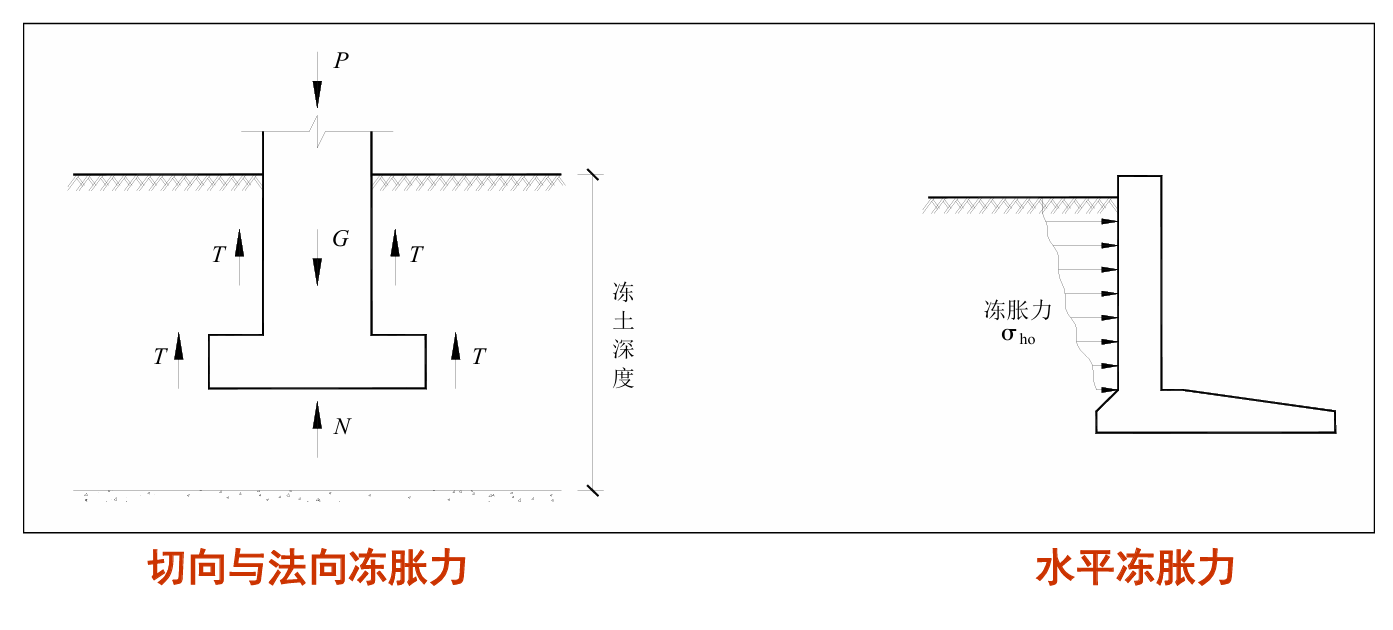
\includegraphics[width=0.7\textwidth]{../figure/1.png}
    \caption{冻胀力作用示意图}
\end{figure}

冻胀力按方向分为法向、切向和水平。切向平行于结构侧面,起到一个提起结构的效果。法向垂直于地面,当达到法向作用的深度,法向力起到一个抬升作用。
水平力起到一个挤压推动的作用,会导致结构水平方向变形或者位移。

\section{冰压力}
\begin{enumerate}
    \item 静冰压力
    \begin{itemize}
        \item 冰堆整体推移
        \item 风和水流作用于大面积冰层
        \item 冰覆盖层受温度变化产生膨胀力
        \item 冰层因水位升降产生竖向作用力
    \end{itemize}

    \item 动冰压力:主要指河流流冰产生的冲击动压力。
\end{enumerate}

\section{撞击力}
通航河流中的桥梁墩台在服役过程中可能遭到船只或漂流物撞击,设计时需予以考虑。

其中,船舶撞击力的影响因素有:
\begin{enumerate}
    \item 环境因素(风浪、气候、水流等)
    \item 船舶特性(船舶类型、尺寸、行进速度、装载情况等)
    \item 桥梁结构因素(桥梁构件的尺寸、形状、材料、质量和抗力等)
    \item 驾驶员反应时间
\end{enumerate}

\ifx\allfiles\undefined
\end{document}
\fi